\section{Experiments}\label{sec:experiments}

In this section we  demonstrate the use of the proposed statistical framework for evaluating a set of VAEs in the context of modelling a statically binarised version of MNIST \citep{deng2012mnist} and the English PTB \citep{marcus1993ptb}.


%\footnote{\url{http://yann.lecun.com/exdb/mnist/}}
%\footnote{\url{https://huggingface.co/datasets/ptb_text_only}} 

\subsection{VAEs}

% Objectives
% Architectures MNIST
% Architectures PTB

\paragraph{Optimisation criteria.} We employ three different optimisation criteria in our experiments that by design relate to the issues highlighted Section \ref{sec:intrinsic}. 
\textbf{$\beta$-VAE} (\textsc{BetaVae}): \citet{higgins2016beta} propose a framework for controlling the capacity of the information bottleneck by adding a hyperparameter $\beta$ to the ELBO objective. \textbf{Info-VAE} (\textsc{InfoVae}): \citet{zhao2017infovae} propose this optimisation criterion to allow for explicitly controlling the balance between accurate posterior inference and maintaining substantial mutual information between the latent and observed variables. We implement this objective as a $\beta$-VAE objective with an additional MMD term, weighted with hyperparameters $\lambda_\text{rate}$ and $\lambda_{\text{MMD}}$ respectively. \textbf{Free bits VAE} (\textsc{FbVae}): to counteract the mutual information between the latent and observed variables to vanish and indirectly stimulate a non-collapsed posterior \citet{kingma2016improved} propose to alter the expected ELBO replacing $R$ by $\max(\lambda_\text{FB}, R)$ in an attempt to enforce a minimum rate.
For both the experiments on MNIST and PTB we select a range of values for $\beta$, $\lambda_\text{rate}$, $\lambda_{\text{MMD}}$ and $\lambda_\text{FB}$, which are listed together with an overview of the criteria in the supplementary material (Section \ref{app:hyperparameters}, Tables \ref{tab:objectives-hp} and \ref{tab:objectives}).

\paragraph{Architectures.} For all experiments we implement a standard VAE with a fully factorised Gaussian approximate posterior $q_{Z|X=x}$ and a standard Gaussian as prior $p_Z$. The dimensionality of the latent space used across all the MNIST experiments is 10 and for all the PTB experiments 32. We describe some important architectural details below and refer the reader to Section \ref{app:architectures} of the supplementary material for more details. {\bf MNIST:} We experiment with two types of observational model. The simple model is a fully factorised product of Bernoulli distributions with gated transposed convolution layers as its main building block (\ie, CNN.T decoder), following \citet{van2018sylvester}. %We will refer to this architecture as the CNN.T decoder. 
The more complex observational model employs a conditional PixelCNN++ architecture \citep{salimans2017pixelcnn++} to achieve an autoregressive product of Bernoulli distributions, following the implementation of \cite{alemi2018fixing}. %We will refer to this architecture as the PixelCNN++ decoder. 
We keep the architecture of the inference model (the \textit{encoder}) fixed and again follow the implementation with gated convolutional layers of \citet{van2018sylvester}. {\bf PTB:} We experiment with an auto-regressive factorisation of the observational model, and follow \cite{li2020optimus} in altering a transformer architecture \citep[RoBERTa;][]{liu2019roberta} to an auto-regressive model that incorporates the latent via two mechanisms: the embedding mechanism and the attention mechanism. To decrease computational overhead we initialise the weights with a distilled checkpoint \citep{Sanh2019DistilBERTAD}. For the encoder we use an original version of the RoBERTa architecture initialised with the same distilled weights.



\subsection{Latent structure models}\label{subsec:bda_models}

Here we describe the latent structure models (LSMs) used to assign lppd to the model samples and control groups outlined in \rsec{approach}. 
%We investigate three models for assessing data fit $q_X \sim p_X$ and one for latent fit $q_Z \sim p_Z$ \cbnote{need a better term for latent fit, prior fit? not to confuse with the latent structure also}.
Their designs and complexity may vary across application domains and be chosen according to the practitioners liking, but we encourage to iteratively build complexity as even simple models can have surprising discriminative power, as we shall see. The graphical representations of our LSMs are shown in Table \ref{tab:BDA_diagrams} in the supplementary material. %We use the letter $c$ across representations to denote the variable that captures the local latent structure we intend to verify. 
It is worth noting that even though LSMs themselves are of generative nature, their ability to act as a generator in a realistic scenarios is simply too limited. But, their latent parameters may capture a data-driven notion of the latent structure at hand which a practitioner may want a more powerful  generator, such as a VAE, to also induce. Moreover, if samples from a VAE do not seem data-like under the LSM's (simple) factorisation, the VAE has surely failed at modelling the complex $q_X$.

%, for heldout samples $\mathcal D'_X$ presumably comply with training samples $\mathcal D_X$ in terms of word frequency.

% \footnote{Consider the example where $\Omega_X$ is the space of English documents, a latent Dirichlet allocation model \citep[LDA;][]{LDA} is not a good generator (\ie, documents sampled from LDA are unordered collections of words), but its latent space captures a data-driven notion of topics which a practitioner may want a powerful  generator, such as a VAE, to also induce. Moreover, if samples from a VAE do not seem data-like under the LDA's factorisation, the VAE has surely failed at modelling $q_X$, for heldout samples $\mathcal D'_X$ presumably comply with training samples $\mathcal D_X$ in terms of word frequency.}

%\wanote{We could remark something on why this makes sense. One might be thinking, if we have a LSM why are we using VAEs? Good LSMs are usually not good generators, good generators (\eg, some VAEs) are not good LSMs. (and ofc,  some excellent generators are not even LVMs.)}

% Digit identity model
\paragraph{MNIST digit identiy model.}
The most obvious latent structure present in the MNIST dataset is that of the digit identity. Assessing whether VAEs capture this structure helps detect severely failed optimisation. To this end we design a simple LSM that is a mixture over 10 components, each of which is defined as a joint over independent Bernoulli distributions with a shared Beta prior to model the pixel values. This can be thought of as a naive Bayes classifier, and, in fact, we supervise it by pre-annotating the MNIST training data with classes predicted using a k-nn classifier (with 96.6\% accuracy).

% \cbnote{citation for mixture model?}\wanote{no need, this is a Bayesian NBC}

% Sequence length model
\paragraph{PTB sequence length model.}

A core property of written text is variability in sequence length. To test whether our VAEs capture this characteristic credibly, we design an LSM that models sentence length under a latent mixture of Poissons (latent components in Figure \ref{fig:ptb_data_model_length_distributions} of the supplement). %Specifically, we choose to model the length as drawn from a mixture of Poissons with a shared Gamma prior.

% \cbnote{the mixture weights are sampled from a DP, do we need to note this? I am still a little vague on DPs... do we need to say "infinite" mixture?}\wanote{I don't think we need that here}

% Topic model
\paragraph{PTB topic model.}
% Checks for LDA \citep{mimno-blei-2011-bayesian}.

Subsequently, we define another LSM to evaluate VAEs fitted on PTB which focuses more on the content of the written text. To this end, we use latent Dirichlet allocation \cite[LDA;][]{blei2003lda} to uncover an underlying topic structure to the text we are modelling in the form of distributions over word count vectors. %This corresponds to a `bag-of-words' view of sentences.

% \cbnote{Do we need to highlight the fact that this again is a simplified view of the data (bow)? And that for PTB this might be complex enough? Perhaps we need to suggest more complex ones? Like the HMM idea?}

% Latent analysis model
% \paragraph{Latent analysis model.}
% Lastly, we design a model to directly compare samples from the prior $p_Z$ with samples from the marginal $q_Z$ of different VAE models. We employ a mixed membership model to model samples from the prior $p_Z$ and models $q_Z$ as groups under the same model. This model deviates slightly from the models defined over the data space as we know the explicit latent structure we seek to be present in the model samples: that of the prior. This allows for a shortcut in the analysis because we can directly compare groups under this model. 

% \cbnote{mixed membership model citations}
% \cbnote{say that in terms of analysis this is an alternative to MMD?}

%Early applications of mixed membership modeling included the admixture model in genetics (Pritchard et al., 2000a), the Grade of Membership model in medical classification studies (Manton et al., 1994b), and the latent Dirichlet allocation model in machine learning (Blei et al., 2003)

\subsection{Analysis}

% Intrinsic evaluation
\begin{figure}
    \centering
    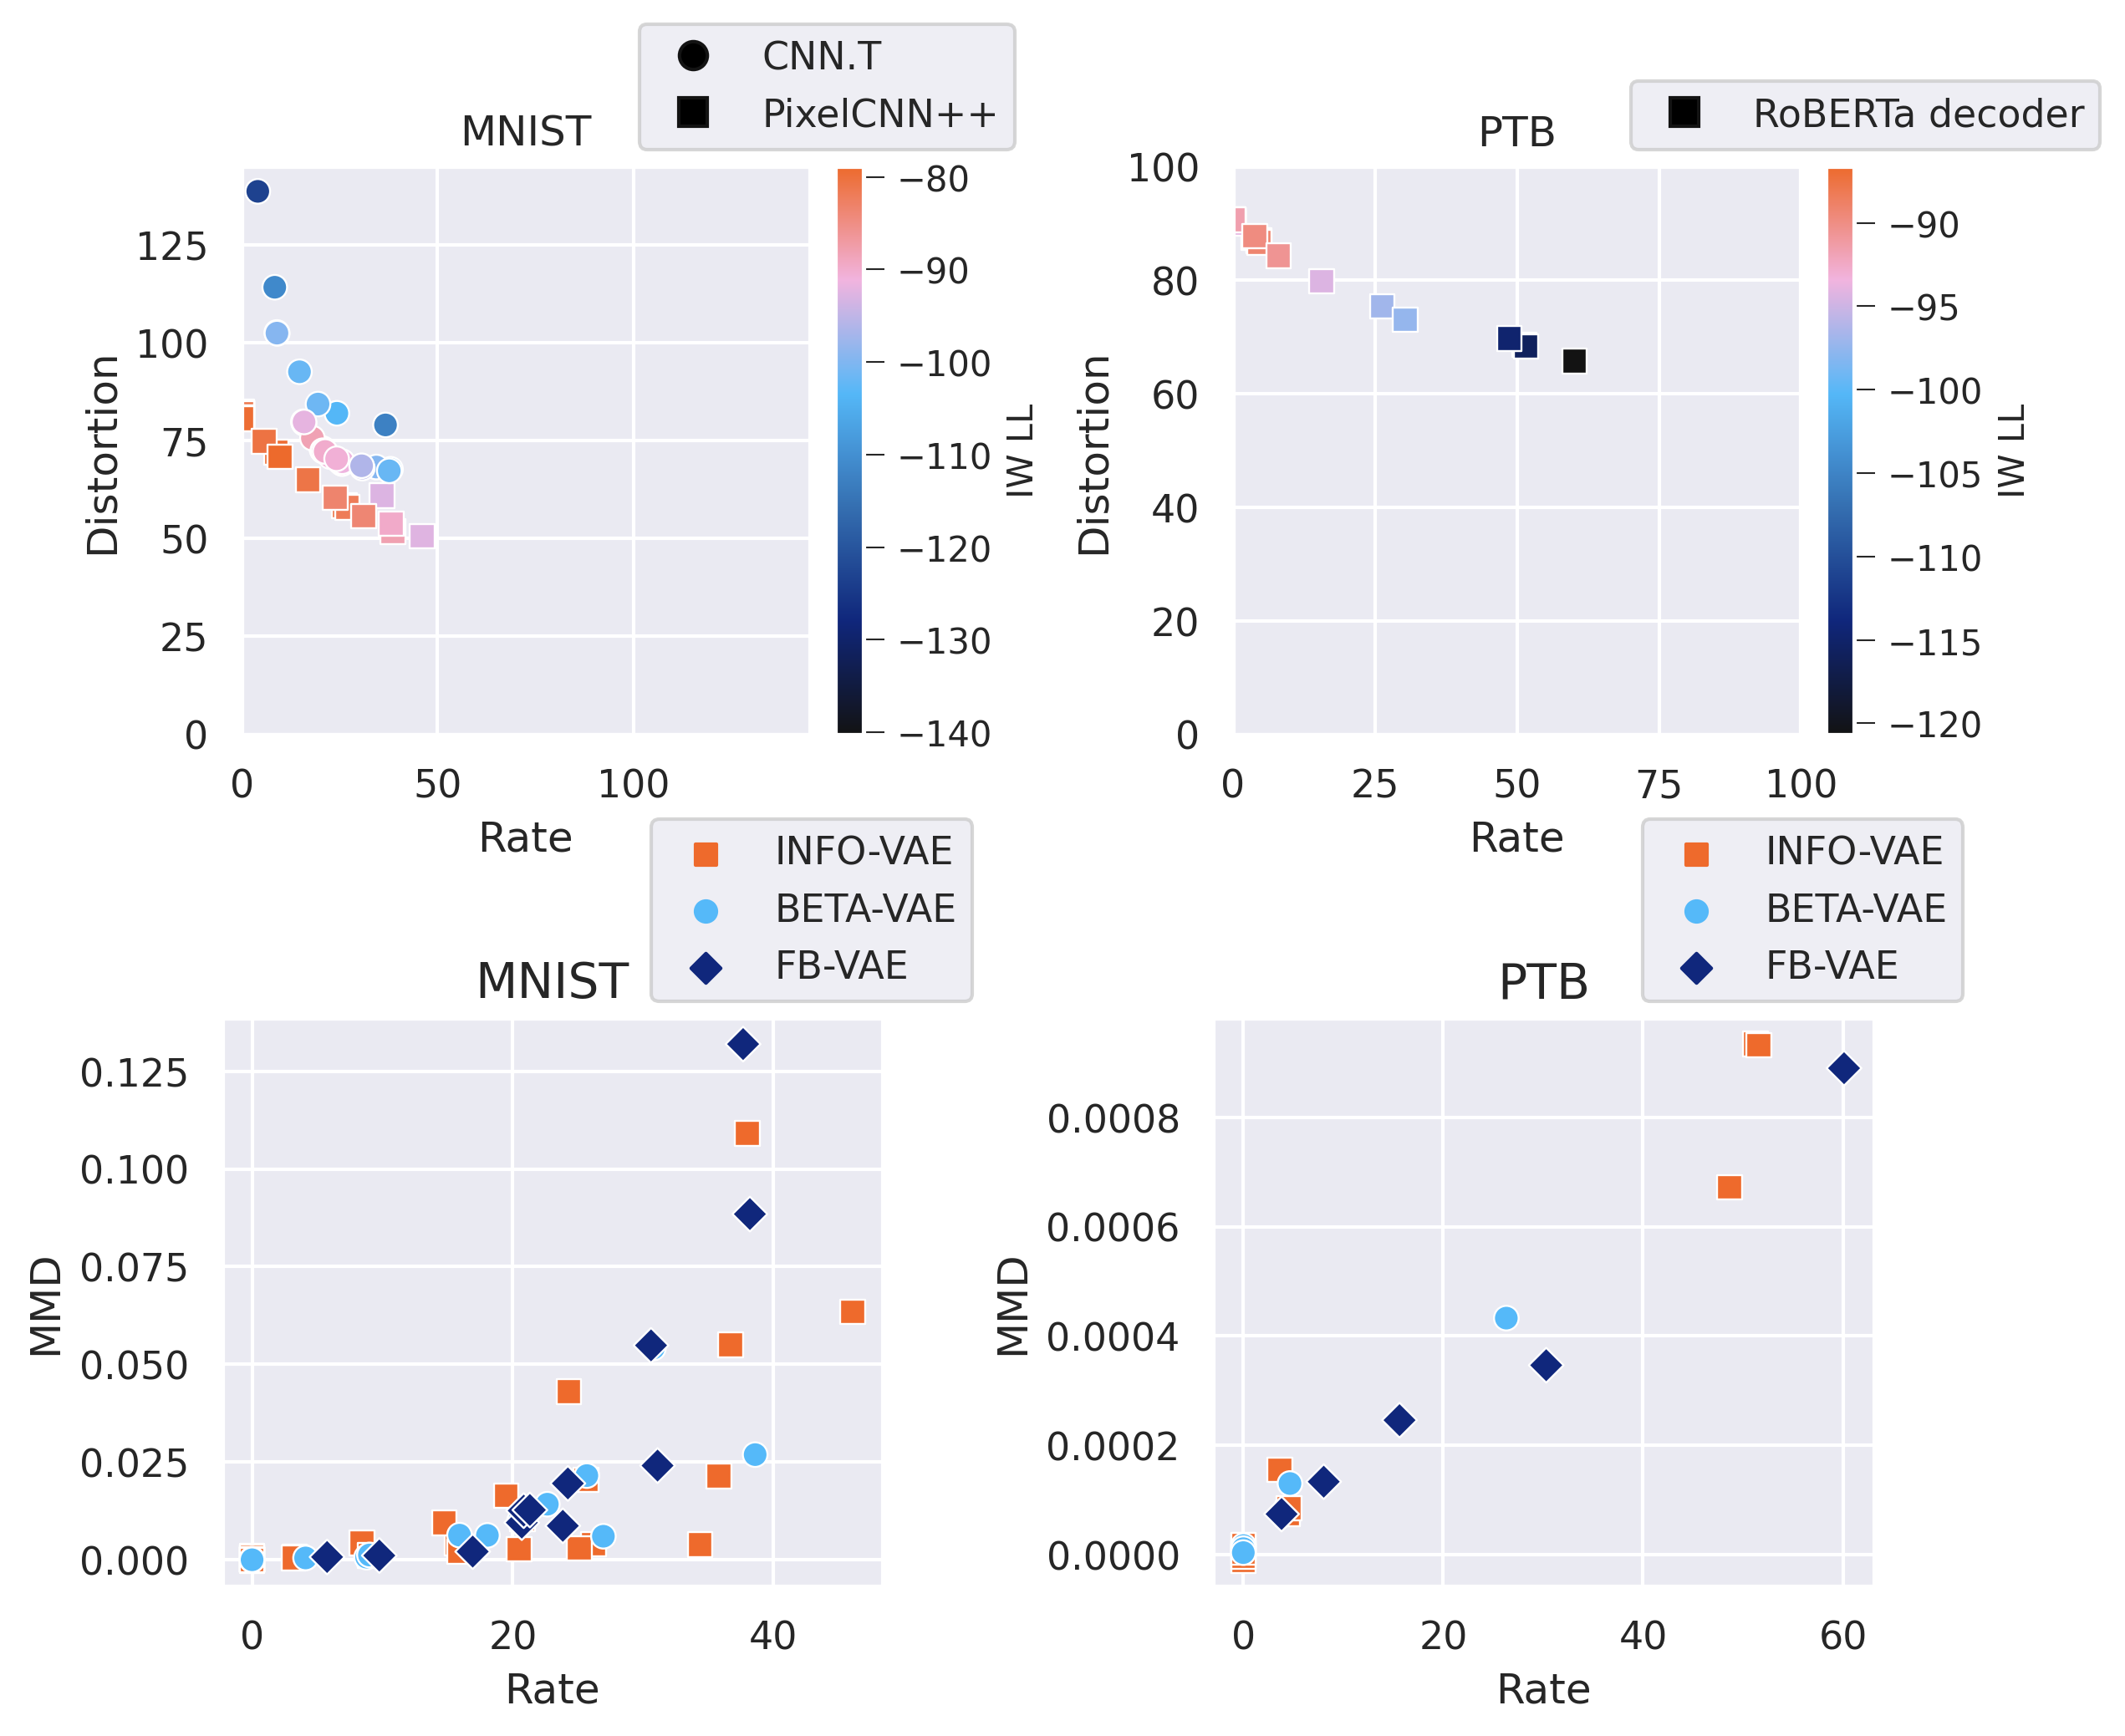
\includegraphics[width=0.5\textwidth]{images/intrinsic_evaluation.png}
    \caption{The intrinsic evaluation results of all experiments.}
    \label{fig:intrinsic-evaluation-plot}
\end{figure}

\paragraph{Intrinsic evaluation.}
Intrinsic evaluation metrics are summarised visually for all experiments in Figure \ref{fig:intrinsic-evaluation-plot}. Full tabular results can be found in the supplementary material (Section \ref{app:intrinsic-evaluation}). For the MNIST CNN.T experiments we see that the trade-off between R and D is defined by a bent curve: the first segment of the curve defines a region where D can be diminished with R efficiently (steep D decrease between experiments) and the second segment of the curve defines a region where the opposite is true. For the PixelCNN++ experiments and all the PTB experiments we observe more typical strong decoder behaviour where the conversion between R and D is an inefficient one for all levels of R that have been recorded in our experiments. In the lower two plots we can observe that for almost all experiments MMD increases with an increase in R. To which extent this happens differs per objective in the MNIST experiments, but for PTB it seems that all objectives act quite similarly in this regard. Additionally, we observe that the MMD scale is quite different for MNIST than for PTB, which makes it hard to tie practical judgements to the consequence of elevated MMD.

% SURPRISAL VALUE DIST PLOTS
\begin{figure*}[t]
     \centering
     \begin{subfigure}{\textwidth}
         \centering
         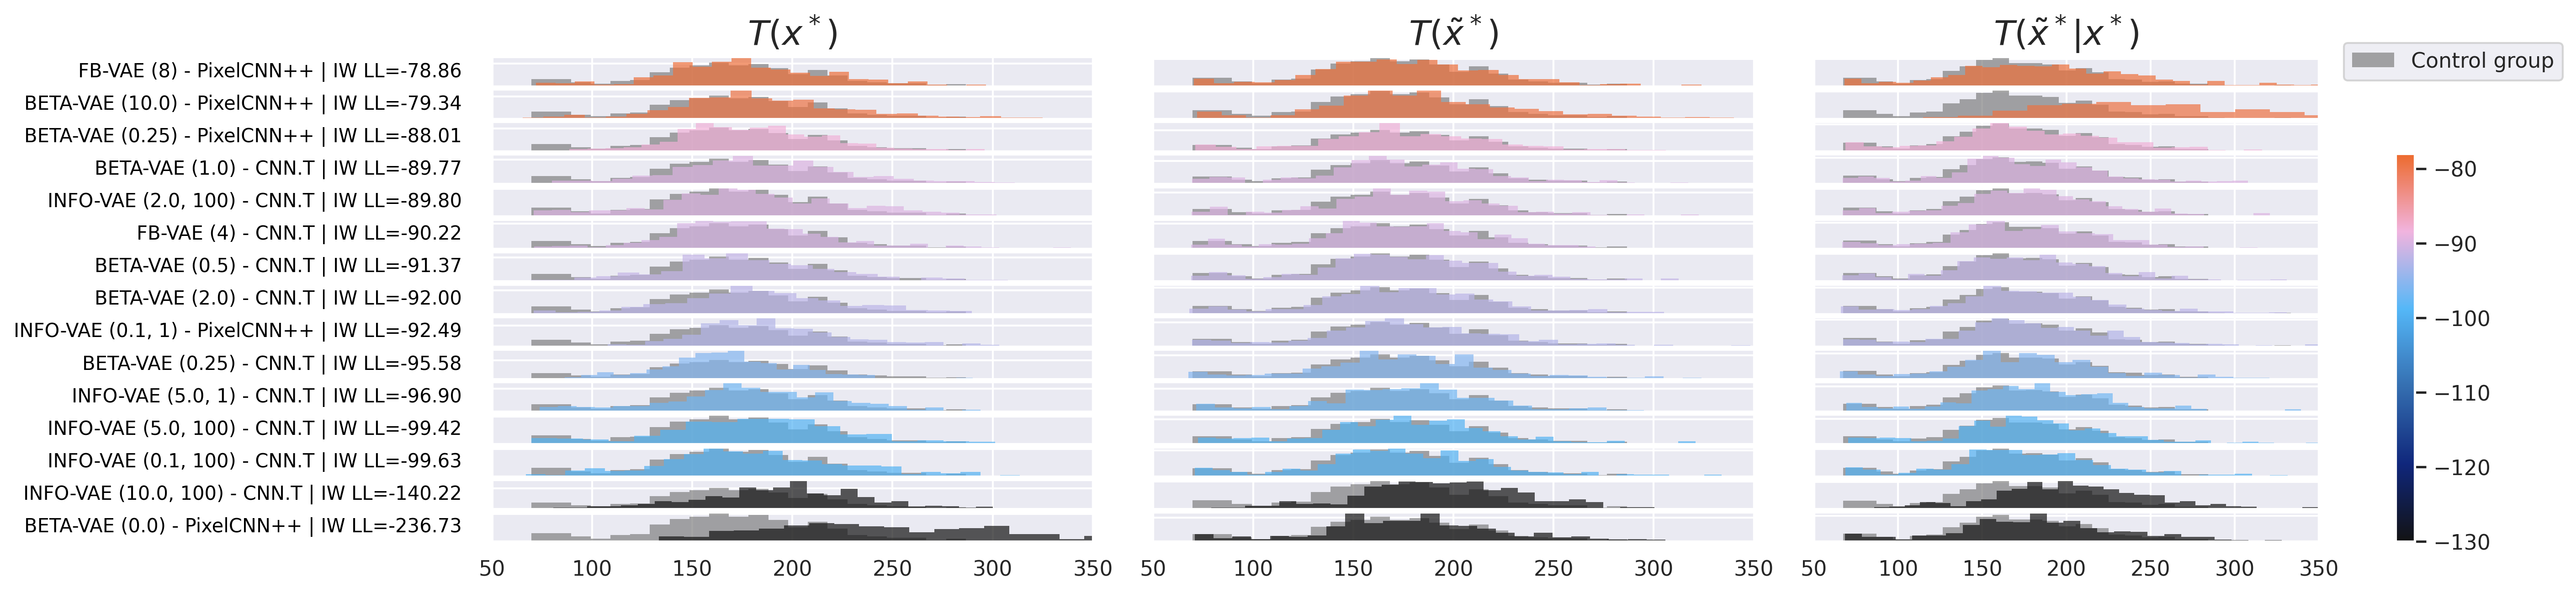
\includegraphics[width=\textwidth]{images/surprisal_dists/mnist_surprisal_dist_SMALL_SELECT.png}
         \caption{MNIST digit identity}
         \label{fig:all-surprisal-dists-sub-mnist}
     \end{subfigure}
    %  \hfill
     \begin{subfigure}{\textwidth}
         \centering
         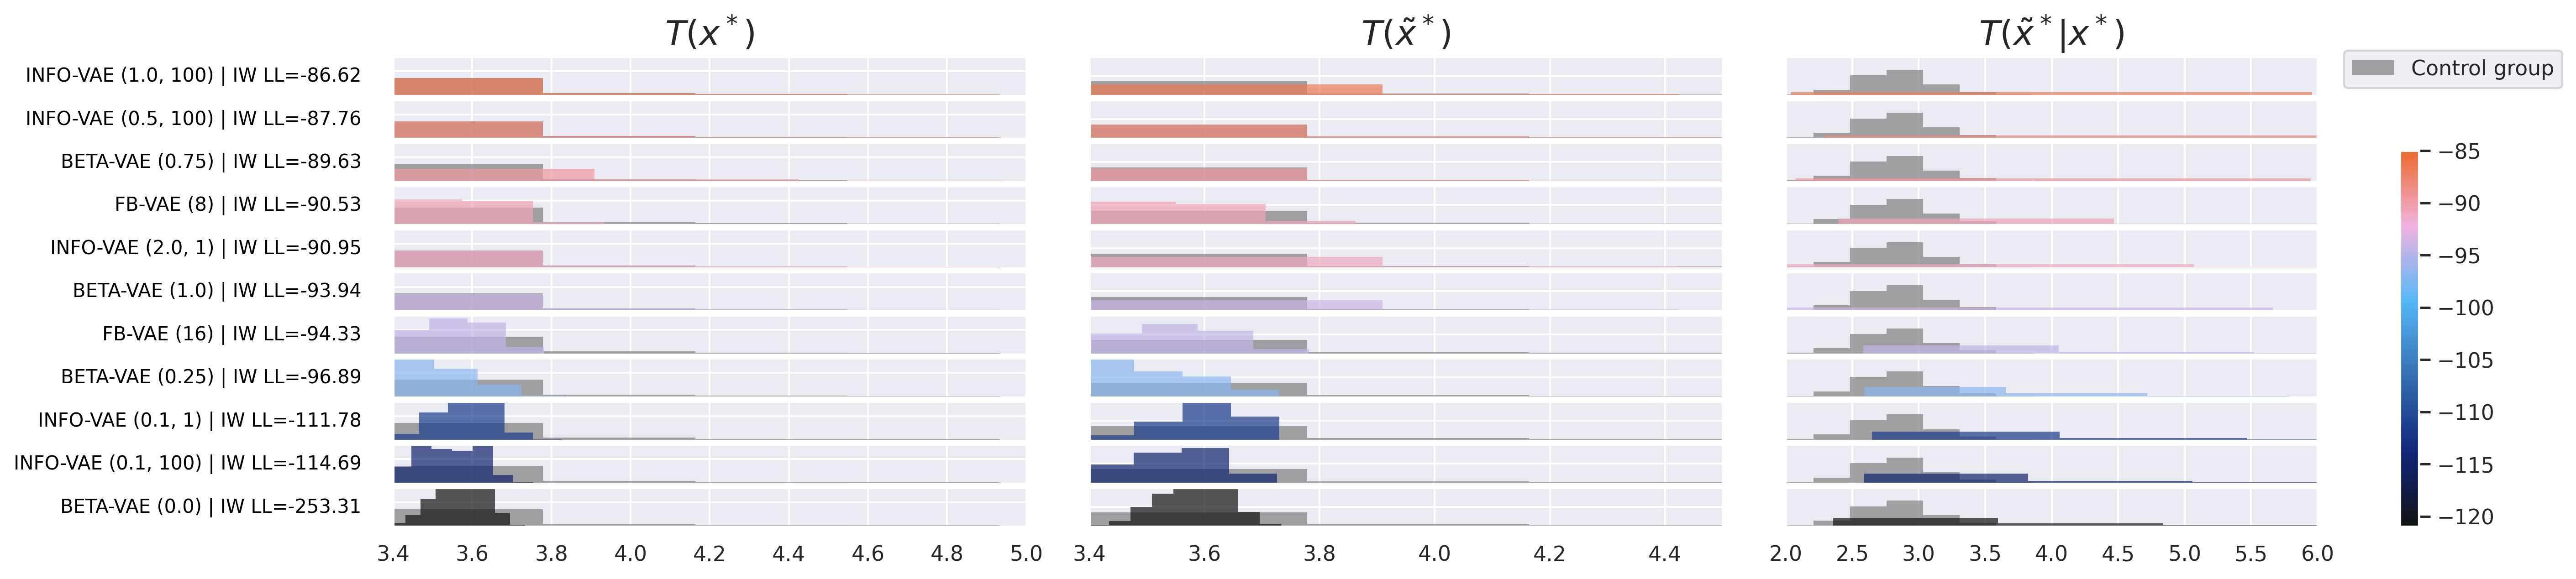
\includegraphics[width=\textwidth]{images/surprisal_dists/ptb_seq_len_surprisal_dist_SMALL_SELECT.png}
         \caption{PTB sequence length}
         \label{fig:all-surprisal-dists-sub-ptb-seq-len}
     \end{subfigure}
    %  \hfill
     \begin{subfigure}{\textwidth}
         \centering
         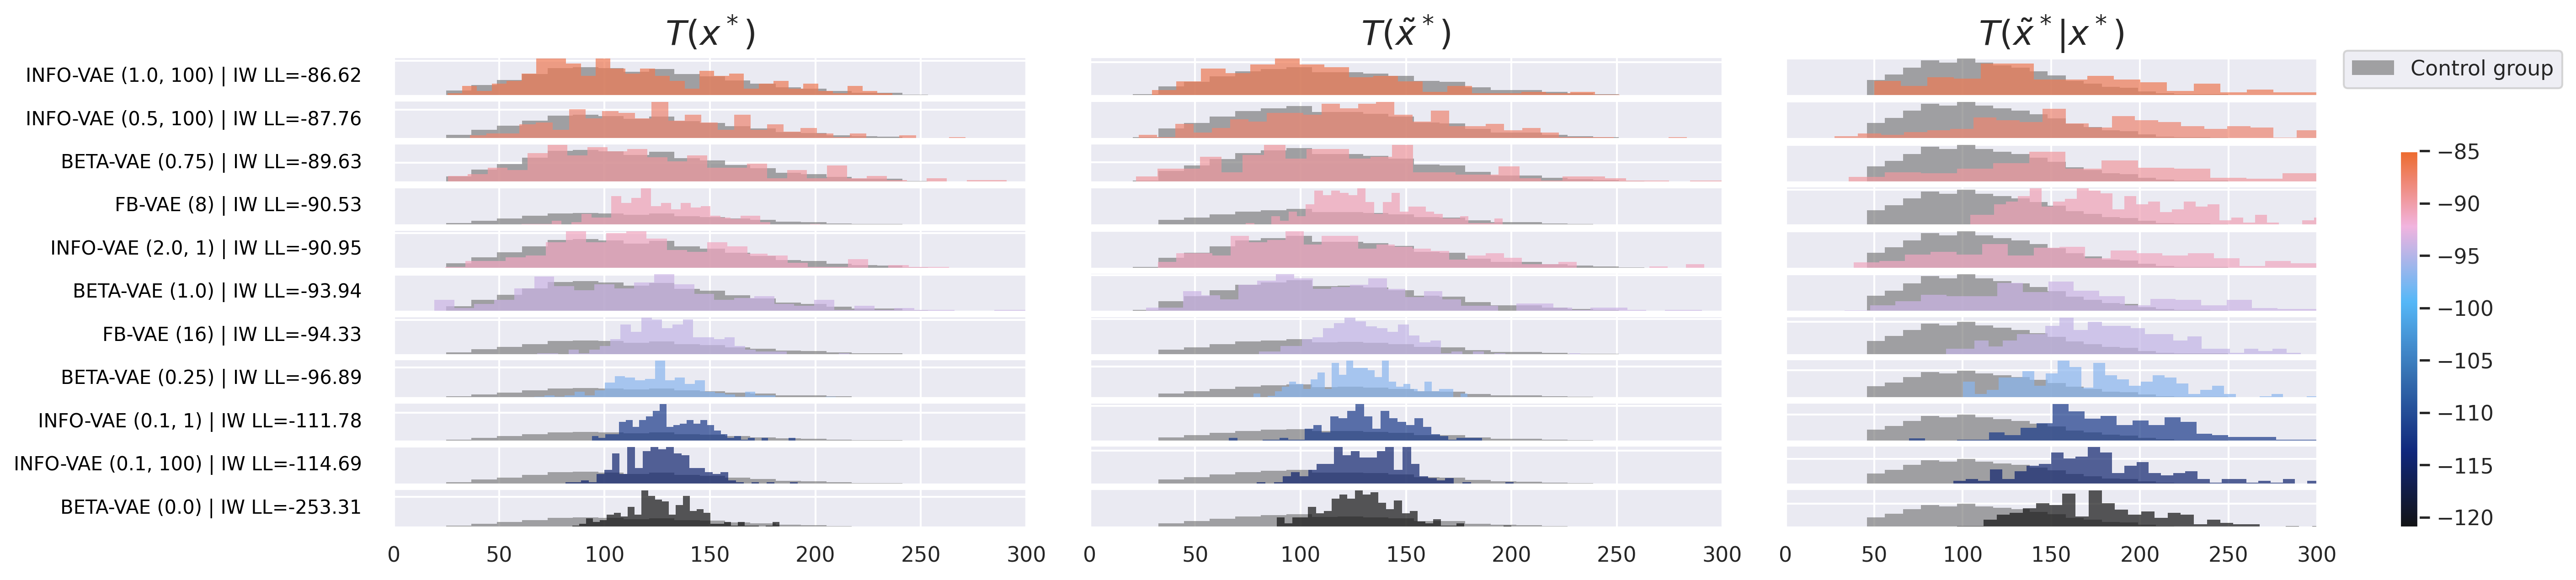
\includegraphics[width=\textwidth]{images/surprisal_dists/ptb_lda_topics_surprisal_dist_SMALL_SELECT.png}
         \caption{PTB topics}
         \label{fig:all-surprisal-dists-sub-ptb-topics}
     \end{subfigure}
        \caption{The three statistics $T(X_*)$, $T(\tilde X_*)$ and $T(\tilde X_*|X_*)$ assessed under the three LSMs visualised for a subset of the experiments together with the distributions of the control groups. The rows are ordered and coloured by IW LL. The experiments are labelled with the objectives according to the following format: \infovae ($\lambda_{\text{rate}}$, $\lambda_{\text{MMD}}$), \betavae ($\beta$) and \fbvae ($\lambda_{\text{FB}}$). For the MNIST experiments we additionally distinguish between decoder types used (CNN.T or PixelCNN++). We refer the reader for full experimental results to the supplementary material (Section \ref{app:latent-structure-models}).}
        \label{fig:all-surprisal-dists}
\end{figure*}

\paragraph{Negative lppd under latent structure model.}
To get an initial overview of the result of our analysis, we plot the histograms of the collected statistics for a subset of the experiments together with those belonging to the control group in Figure \ref{fig:all-surprisal-dists}. We sort and colour the rows of the plots according to IW LL. Plots with all experiments can be found in the supplementary material (Section \ref{app:latent-structure-models}). By inspecting the distributions we can make a few general observations. Primarily, it can be observed that the ordering according to IW LL does not generally correspond to the perceived divergences in histograms from the control group across statistics. On both ends of the IW LL spectrum we can find distributional discrepancies with respect to to the control group. Conversely, we can perceive differences in the distribution of statistics for models that are nearly identical in terms of IW LL. For the MNIST digit identity model (Figure \ref{fig:all-surprisal-dists-sub-mnist}), for example, we can see that the best models in terms of statistics distributions seem to reside around an IW LL of $-90$. In fact, we can even distinguish models in that range by inspecting the histograms closely. We can, for example, distinguish them in their ability to model the multi-modal nature of the control group with regards to $T(X_*)$: the \infovae (2.0, 100) MNIST experiment seems to capture the small chunk of probability mass at the lower end of the spectrum better than the experiment above and below it. Similarly, for the PTB topic model (Figure \ref{fig:all-surprisal-dists-sub-ptb-topics}) we can for instance visually appreciate differences between the \fbvae (8.0) experiment and its row-wise neighbours, while they have nearly identical average IW LL estimates.

% KL PLOTS
\begin{figure*}[ht]
     \centering
     \begin{subfigure}{\textwidth}
         \centering
         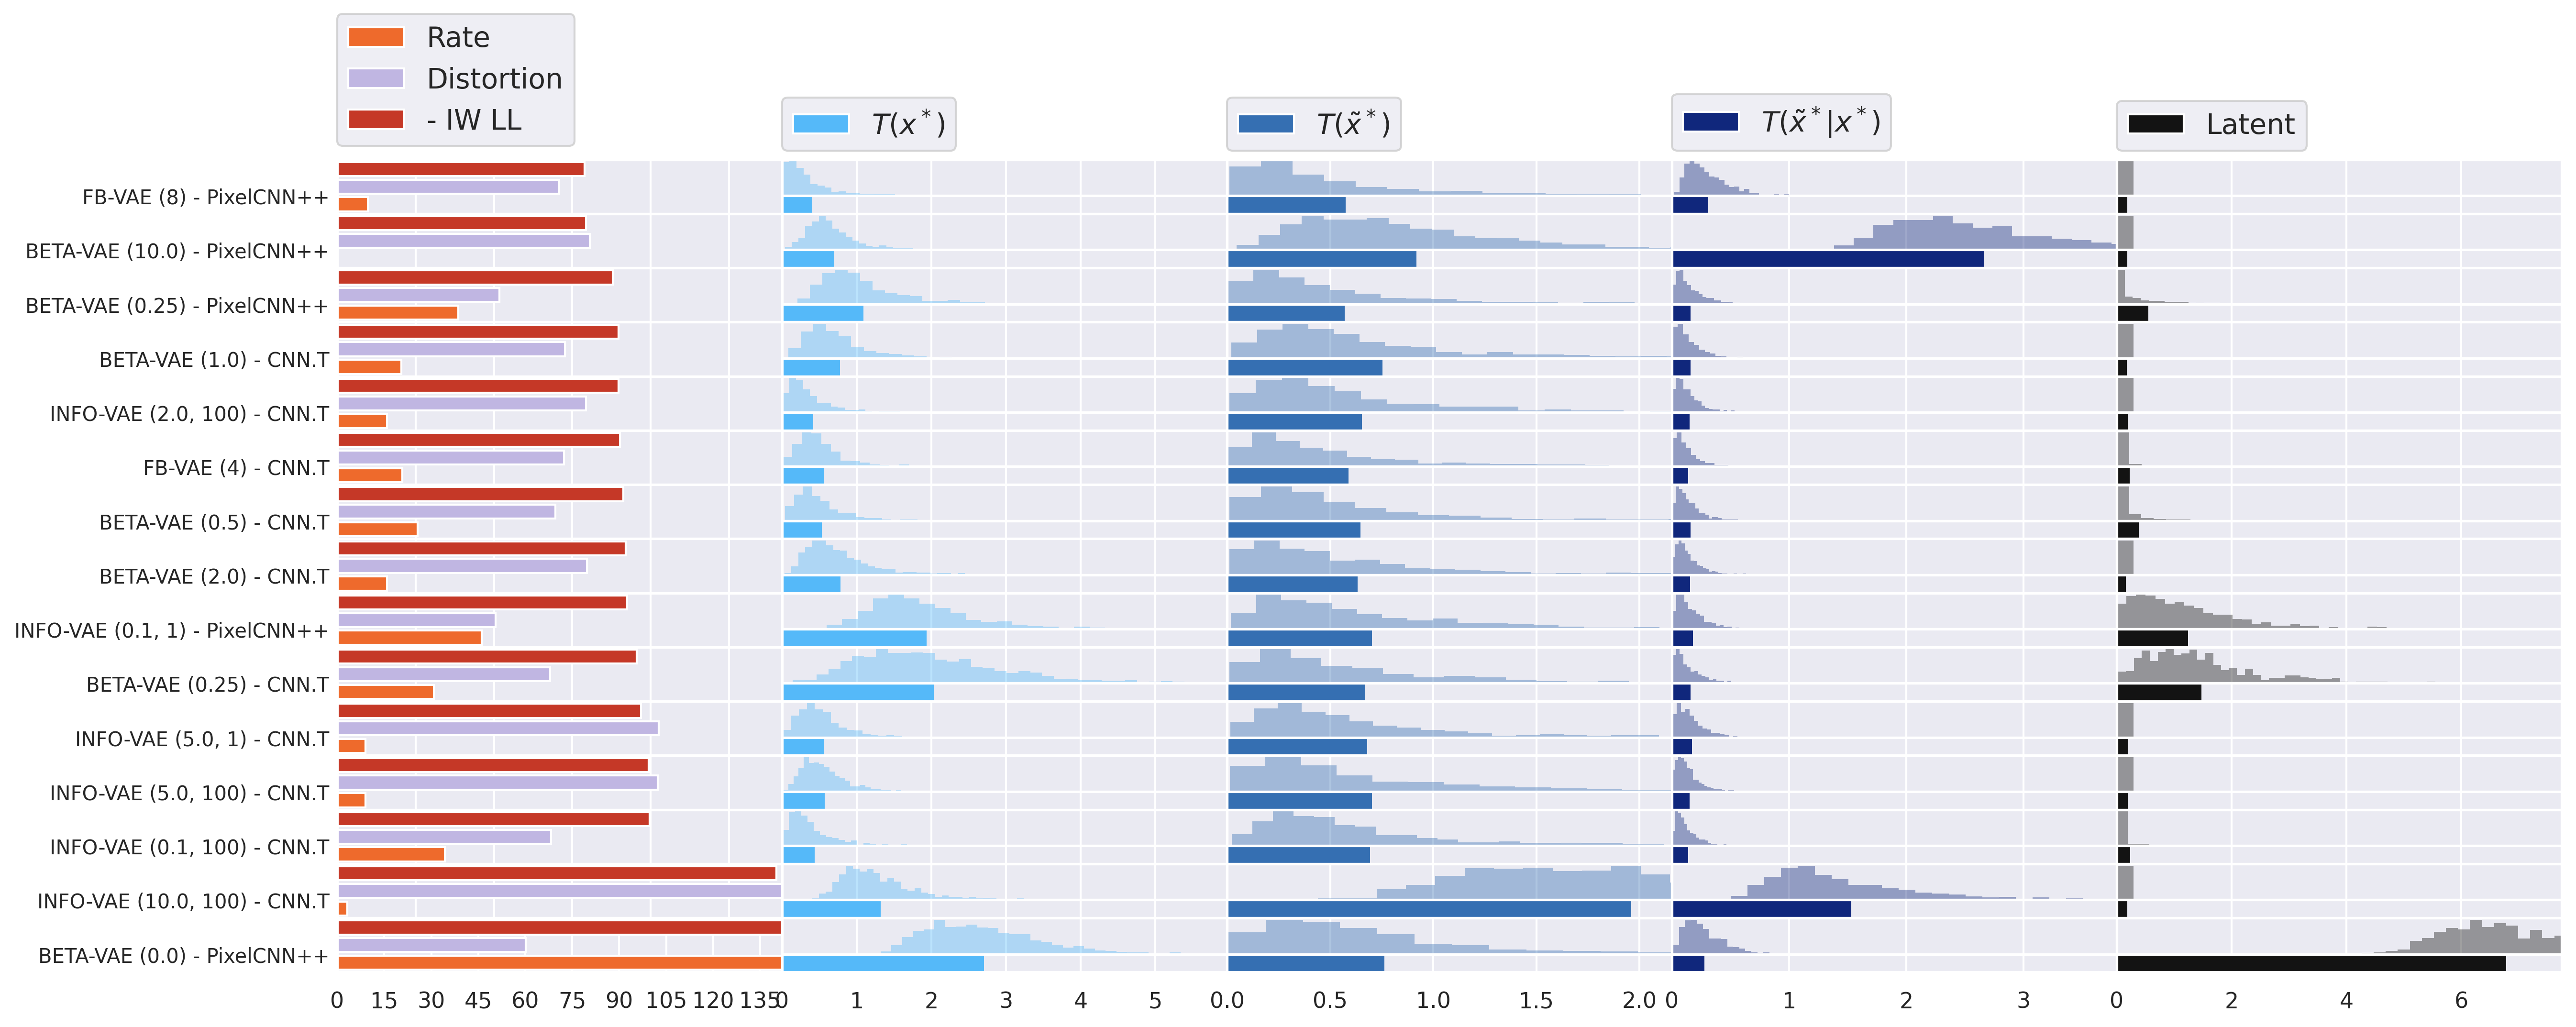
\includegraphics[width=\textwidth]{images/kl_plots/mnist_selection_True.png}
         \caption{MNIST digit identity}
         \label{fig:all-kl-plots-sub-mnist}
     \end{subfigure}
    %  \hfill
     \begin{subfigure}{\textwidth}
         \centering
         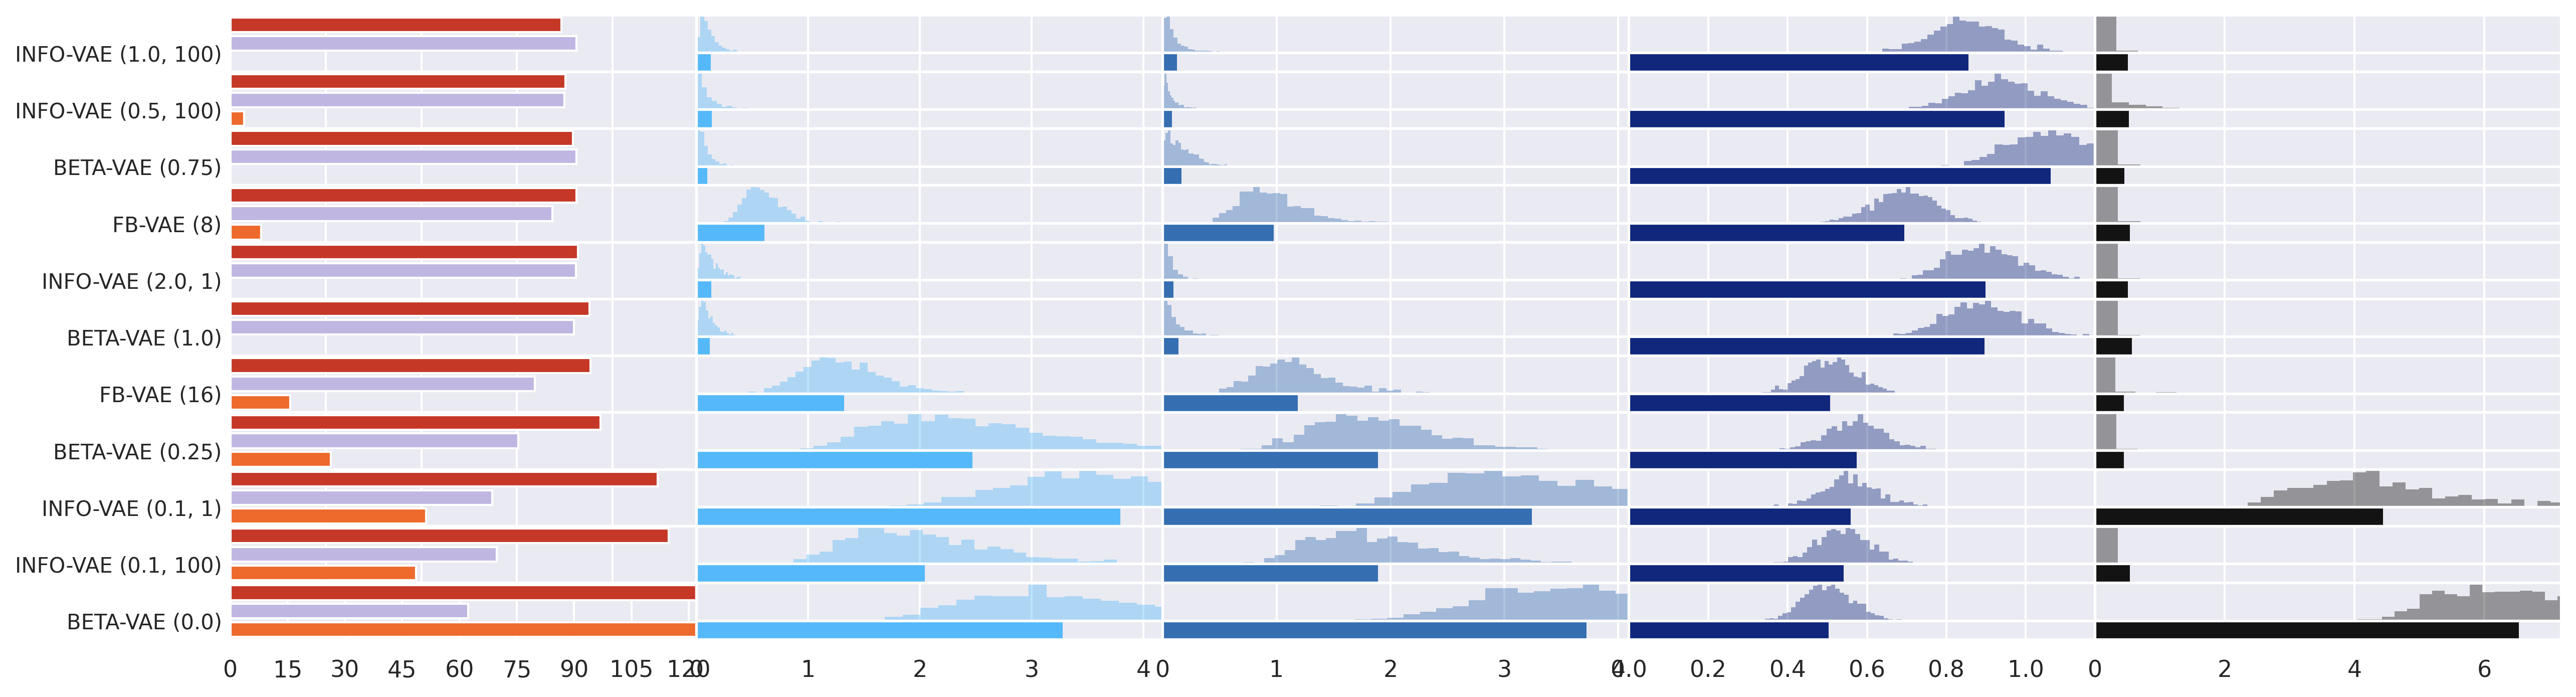
\includegraphics[width=\textwidth]{images/kl_plots/ptb_sequence_len_selection_True.png}
         \caption{PTB sequence length}
         \label{fig:all-kl-plots-sub-ptb-seq-len}
     \end{subfigure}
    %  \hfill
     \begin{subfigure}{\textwidth}
         \centering
        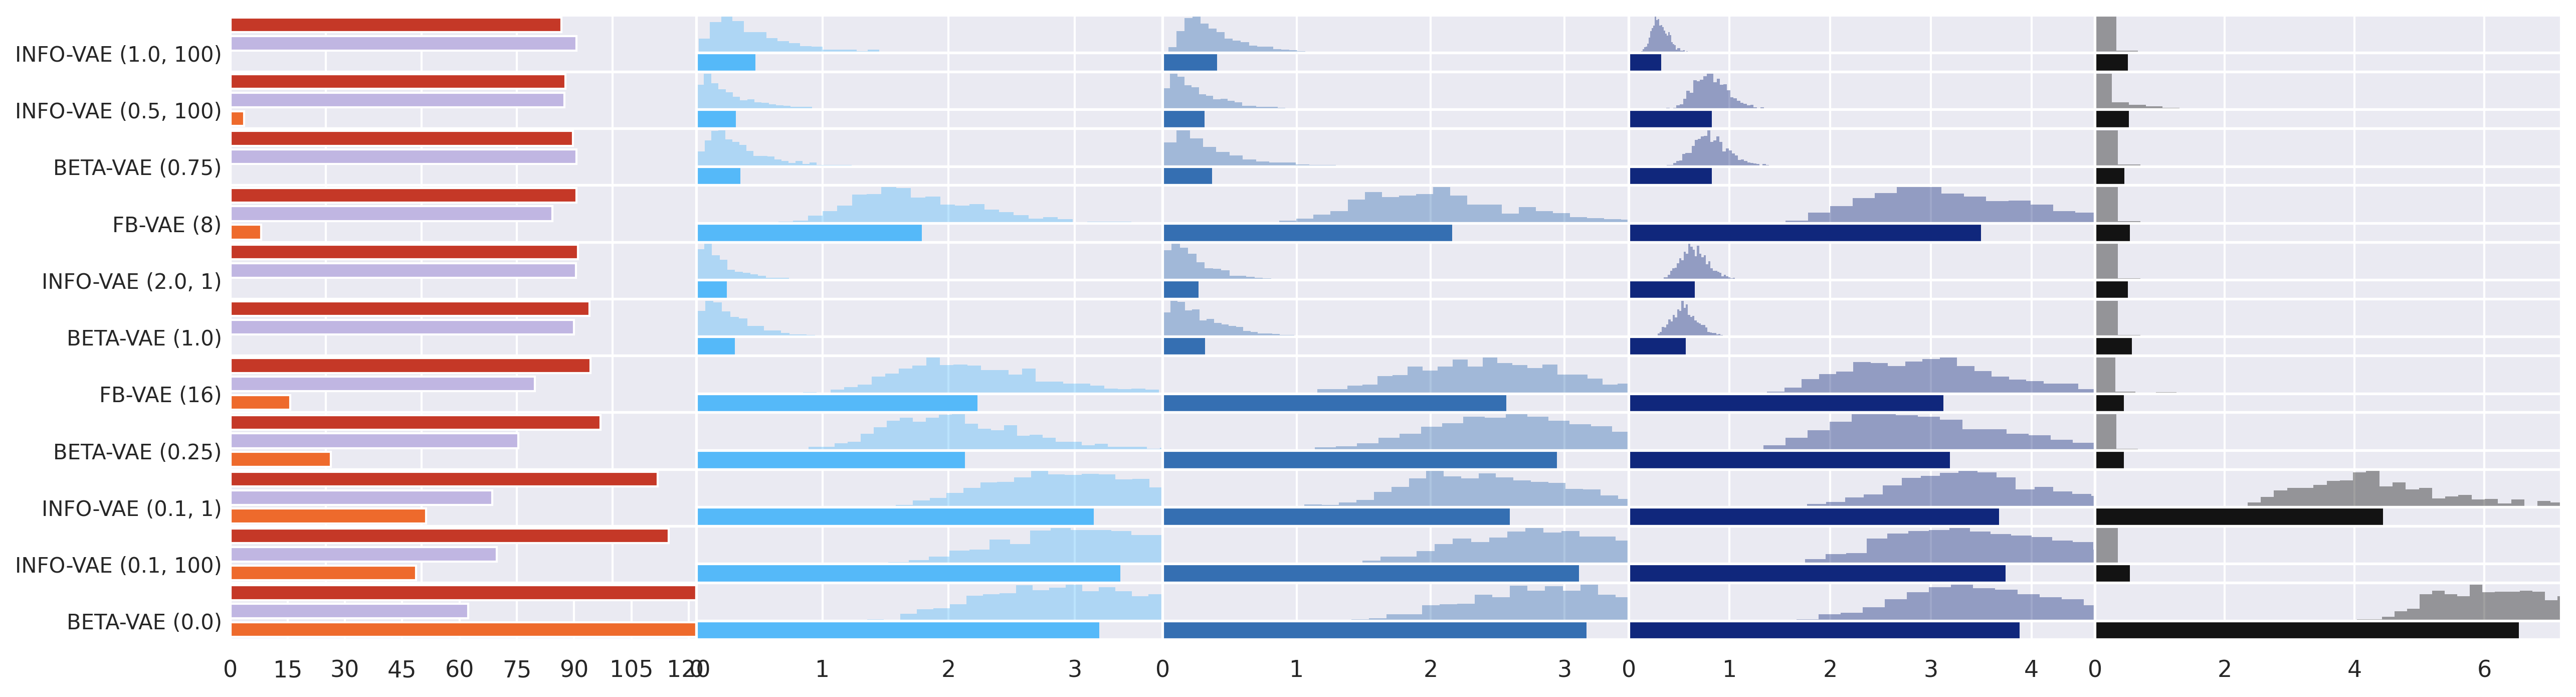
\includegraphics[width=\textwidth]{images/kl_plots/ptb_topics_selection_True.png}
         \caption{PTB topics}
         \label{fig:all-kl-plots-sub-ptb-topics}
     \end{subfigure}
        \caption{A summarising view of our analysis of a subset of the experiments. The leftmost column shows the intrinsic evaluation metrics for reference. The next three columns show estimated divergences from the control group under our analysis model. The rightmost column shows the estimated divergence from $q_Z$ to $p_Z$. Full experimental results can be found in the supplementary material (Section \ref{app:kl-plots}). The horizontal bars denote the average value of the sampled posterior divergences plotted as histograms. The experiments are labelled with the objectives according to the following format: \infovae ($\lambda_{\text{rate}}$, $\lambda_{\text{MMD}}$), \betavae ($\beta$) and \fbvae ($\lambda_{\text{FB}}$). For the MNIST experiments we additionally distinguish between decoder type used: CNN.T or PixelCNN++.}
        \label{fig:all-kl-plots}
\end{figure*}

% More details on these models and plots that validate their fit can be found in Section \ref{app:dp-models} of the supplementary material. 

\paragraph{Posterior KL upperbound.} Figure \ref{fig:all-kl-plots} is a summary of the analysis. It shows intrinsic evaluation metrics (1st column) alongside the estimated discrepancies relative to the control groups under the analysis models as described in Section \ref{sec:approach} for a subset of the experiments. Full results can be found in the supplementary material Section \ref{app:kl-plots}. The next three columns correspond to the discrepancies between distributions of the three lppd statistics in data space and the rightmost column shows the discrepancy between prior samples and samples from the inference model averaged under $\mathcal H_X$.
% Observations MNIST
For the {\bf digit identity model}, we can observe that low R models have a high average divergence to the data group in terms of the conditional statistic $T(\tilde X_*|X_*)$. This aligns with the intuition that these models fail to capture information on the digit identity in the latent space. Additionally, we can observe that increased R often coincides with larger discrepancy along the $T(X_*)$ and $T(\tilde X_*)$ statistics. 
% Setting beta (or equivalently l_rate too high) can have compromising effects on modelling capabilities (\infovae, 10.0, 100.0)
% High rate compromises the digit identity structure, for example as seen with (FB, 40.0)
% Observations PTB sequence length
On {\bf PTB sequence length}, most models do not perform well in terms of encoding length in the latent space as recorded by the discrepancy along the $T(\tilde X_*|X_*)$ dimension, with the exception of high R models that seem to encode it to some extent. Models with low R (and collapsed posteriors) model length unconditionally as you might expect from large transformer based language models. 
% WILKER comment: For length, we can further say. Not capturing length in latent is not per se a problem (ofc). Still, we can detect failure to capture length by other means (eg, autoregressiveness), as again, pushing rate higher while staying in a reasonable IWL range hurts unconditional_unconditional and unconditional_conditional.
% that is basically scenario C in the marginal KL diagrams right?
% Observations for PTB topic model
The {\bf PTB latent topics} paint a rather different picture. The tendency for high R and the conditional statistic $T(\tilde X_*|X_*)$ is flipped: higher R only harms along this axis and correspondingly along the other statistical axes. 

% INFO VAE MMD
For both MNIST and PTB, \infovae with high enough $\lambda_{\text{MMD}}$ weight can diminish divergence from the prior as measured by the latent analysis model. This does not, however, translate in consistent effects in the data space.
% Additionally: if l_MMD is too low, its does not diminish discrepancy

% WILKER comment: For PTB, we can say these VAEs do not encode length in latent space. Some do encode topics (in an LDA sense). Many that are barely distinguishable intrinsically, perform worse along some of our statistics. The typical heuristic of pushing rate a bit higher while staying in a reasonable IWL ballpark clearly hurts the models along most of our statistics